\PassOptionsToPackage{usenames}{color}
\documentclass[11pt,a4paper]{article}

\usepackage{relsize} % relative font sizes (e.g. \smaller). must precede ACL style
\usepackage{style/acl2015}
\usepackage[colorlinks=true,linkcolor=black,citecolor=black,filecolor=black,urlcolor=black]{hyperref}
\usepackage{natbib}

%\usepackage{times}
%\usepackage{latexsym}

\usepackage{microtype}
\usepackage{ dsfont }
\usepackage[boxed]{algorithm2e}
\renewcommand\AlCapFnt{\small}
\usepackage[small,bf,skip=5pt]{caption}
\usepackage{sidecap} % side captions
\usepackage{rotating}	% sideways
% \usepackage[pdftex]{graphicx}

% Italicize subparagraph headings
\usepackage{titlesec}
\titleformat*{\subparagraph}{\itshape}
\titlespacing{\subparagraph}{%
  1em}{%              left margin
  0pt}{% space before (vertical)
  1em}%               space after (horizontal)

% Numbered Examples and lists
\usepackage{lingmacros}
\newcommand{\exref}[1]{(\ref{#1})} % numbered example

\usepackage[shortlabels]{enumitem} % customizable lists
\setitemize{noitemsep,topsep=0em,leftmargin=*}
\setenumerate{noitemsep,leftmargin=0em,itemindent=13pt,topsep=0em}

\usepackage{xspace}
\usepackage{xparse} % for fancy custom macros (\NewDocumentEnvironment, etc.)

\newcommand{\indicator}[1]{I_{\{#1\}}} %{\mathds{1}_{\{#1\}}}


\usepackage{textcomp}
% \usepackage{arabtex} % must go after xparse, if xparse is used!
%\usepackage{utf8}
% \setcode{utf8} % use UTF-8 Arabic
% \newcommand{\Ar}[1]{\RL{\novocalize #1}} % Arabic text

\usepackage{framed}

\usepackage{listings}

\lstset{
  basicstyle=\itshape,
  xleftmargin=3em,
  aboveskip=0pt,
  belowskip=-3pt, %-.5\baselineskip, % correct for extra paragraph break inserted after listing
  literate={->}{$\rightarrow$}{2}
           {α}{$\alpha$}{1}
           {δ}{$\delta$}{1}
           {(}{$($}{1}
           {)}{$)$}{1}
           {[}{$[$}{1}
           {]}{$]$}{1}
           {|}{$|$}{1}
           {+}{\ensuremath{^+}}{1}
           {*}{\ensuremath{^*}}{1}
}

\usepackage{amssymb}	%amsfonts,eucal,amsbsy,amsthm,amsopn
\usepackage{amsmath}

\usepackage{mathptmx}	% txfonts
\usepackage[scaled=.8]{beramono}
\usepackage[scaled=.85]{helvet}
\usepackage[T1]{fontenc}
\usepackage[utf8x]{inputenc}

\usepackage{MnSymbol}	% must be after mathptmx

\usepackage{latexsym}





% Tables
\usepackage{array}
\usepackage{multirow}
\usepackage{booktabs} % pretty tables
\usepackage{multicol}
\usepackage{footnote}
\newcolumntype{H}{>{\setbox0=\hbox\bgroup}c<{\egroup}@{}} % hidden column


\usepackage{url}
\usepackage[usenames]{color}
\usepackage{xcolor}

% colored frame box
\newcommand{\cfbox}[2]{%
    \colorlet{currentcolor}{.}%
    {\color{#1}%
    \fbox{\color{currentcolor}#2}}%
}

\usepackage[normalem]{ulem} % \uline
\usepackage{colortbl}
\usepackage{graphicx}
\usepackage{subcaption}
%\usepackage{tikz-dependency}
\usepackage{tikz}
%\usepackage{tree-dvips}
\usetikzlibrary{arrows,positioning,calc} 

\DeclareMathOperator*{\argmax}{arg\,max}
\DeclareMathOperator*{\argmin}{arg\,min}
%\setlength\titlebox{6.5cm}    % Expanding the titlebox
\setlength\titlebox{5.5cm}    % Expanding the titlebox

\usepackage{nameref}
\usepackage{cleveref}

% use \S for all references to all kinds of sections, and \P to paragraphs
% (sadly, we cannot use the simpler \crefname{} macro because it would insert a space after the symbol)
\crefformat{part}{\S#2#1#3}
\crefformat{chapter}{\S#2#1#3}
\crefformat{section}{\S#2#1#3}
\crefformat{subsection}{\S#2#1#3}
\crefformat{subsubsection}{\S#2#1#3}
\crefformat{paragraph}{\P#2#1#3}
\crefformat{subparagraph}{\P#2#1#3}
%\crefmultiformat{part}{\S#2#1#3}{ and~\S#2#1#3}{, \S#2#1#3}{, and~\S#2#1#3}
%\crefmultiformat{chapter}{\S#2#1#3}{ and~\S#2#1#3}{, \S#2#1#3}{, and~\S#2#1#3}
\crefmultiformat{section}{\S#2#1#3}{ and~\S#2#1#3}{, \S#2#1#3}{, and~\S#2#1#3}
\crefmultiformat{subsection}{\S#2#1#3}{ and~\S#2#1#3}{, \S#2#1#3}{, and~\S#2#1#3}
\crefmultiformat{subsubsection}{\S#2#1#3}{ and~\S#2#1#3}{, \S#2#1#3}{, and~\S#2#1#3}
\crefmultiformat{paragraph}{\P\P#2#1#3}{ and~#2#1#3}{, #2#1#3}{, and~#2#1#3}
\crefmultiformat{subparagraph}{\P\P#2#1#3}{ and~#2#1#3}{, #2#1#3}{, and~#2#1#3}
%\crefrangeformat{part}{\mbox{\S\S#3#1#4--#5#2#6}}
%\crefrangeformat{chapter}{\mbox{\S\S#3#1#4--#5#2#6}}
\crefrangeformat{section}{\mbox{\S\S#3#1#4--#5#2#6}}
\crefrangeformat{subsection}{\mbox{\S\S#3#1#4--#5#2#6}}
\crefrangeformat{subsubsection}{\mbox{\S\S#3#1#4--#5#2#6}}
\crefrangeformat{paragraph}{\mbox{\P\P#3#1#4--#5#2#6}}
\crefrangeformat{subparagraph}{\mbox{\P\P#3#1#4--#5#2#6}}
% for \label[appsec]{...}
\crefname{part}{Part}{Parts}
\Crefname{part}{Part}{Parts}
\crefname{chapter}{ch.}{ch.}
\Crefname{chapter}{Ch.}{Ch.}
\crefname{figure}{figure}{figures}
\crefname{appsec}{appendix}{appendices}
\Crefname{appsec}{Appendix}{Appendices}
\crefname{algocf}{algorithm}{algorithms}
\Crefname{algocf}{Algorithm}{Algorithms}
\crefname{enums,enumsi}{example}{examples}
\Crefname{enums,enumsi}{Example}{Examples}
\crefname{}{example}{examples} % lingmacros \toplabel has no internal name for the kind of label
\Crefname{}{Example}{Examples}
\crefformat{enums}{(#2#1#3)}
\crefformat{enumsi}{(#2#1#3)}
\crefformat{}{(#2#1#3)}
\crefrangeformat{enums}{\mbox{(#3#1#4--#5#2#6)}}
\crefrangeformat{enumsi}{\mbox{(#3#1#4--#5#2#6)}}

\ifx\creflastconjunction\undefined%
\newcommand{\creflastconjunction}{, and\nobreakspace} % Oxford comma for lists
\else%
\renewcommand{\creflastconjunction}{, and\nobreakspace} % Oxford comma for lists
\fi%

\newcommand*{\Fullref}[1]{\hyperref[{#1}]{\Cref*{#1}: \nameref*{#1}}}
\newcommand*{\fullref}[1]{\hyperref[{#1}]{\cref*{#1}: \nameref{#1}}}
\newcommand{\fnref}[1]{fn.~\ref{#1}} % don't use \cref{} due to bug in (now out-of-date) cleveref package w.r.t. footnotes
\newcommand{\Fnref}[1]{Fn.~\ref{#1}}


\newcommand{\backtick}[0]{\textasciigrave}


\NewDocumentEnvironment{itmize}{}{\begin{itemize}[noitemsep]}{\end{itemize}}
\NewDocumentEnvironment{enumrate}{}{\begin{enumerate}[noitemsep]}{\end{enumerate}}
\let\Item\item
\renewcommand\enddescription{\endlist\global\let\item\Item}
\NewDocumentEnvironment{describe}{}{\renewcommand\item[1][]{\Item \textbf{##1:} }\begin{itemize}}{\end{itemize}}
\NewDocumentEnvironment{edescribe}{}{\renewcommand\item[1][]{\Item \textbf{##1:} }\begin{enumerate}}{\end{enumerate}}


% Author comments
\usepackage{color}
\newcommand\bmmax{0} % magic to avoid 'too many math alphabets' error
\usepackage{bm}
\definecolor{orange}{rgb}{1,0.5,0}
\definecolor{mdgreen}{rgb}{0.05,0.6,0.05}
\definecolor{mdblue}{rgb}{0,0,0.7}
\definecolor{dkblue}{rgb}{0,0,0.5}
\definecolor{dkgray}{rgb}{0.3,0.3,0.3}
\definecolor{slate}{rgb}{0.25,0.25,0.4}
\definecolor{gray}{rgb}{0.5,0.5,0.5}
\definecolor{ltgray}{rgb}{0.7,0.7,0.7}
\definecolor{purple}{rgb}{0.7,0,1.0}
\definecolor{lavender}{rgb}{0.65,0.55,1.0}

% Settings for algorithm listings
% \lstset{
%   language=Python,
%   upquote=true,
%   showstringspaces=false,
%   formfeed=\newpage,
%   tabsize=1,
%   commentstyle=\itshape\color{lavender},
%   basicstyle=\small\smaller\ttfamily,
%   morekeywords={lambda},
%   emph={upward,downward,tc},
%   emphstyle=\underbar,
%   aboveskip=0cm,
%   belowskip=-.5cm
% }
%\renewcommand{\lstlistingname}{Algorithm}


\newcommand{\ensuretext}[1]{#1}
\newcommand{\cjdmarker}{\ensuretext{\textcolor{red}{\ensuremath{^{\textsc{CJ}}_{\textsc{D}}}}}}
\newcommand{\nssmarker}{\ensuretext{\textcolor{magenta}{\ensuremath{^{\textsc{NS}}_{\textsc{S}}}}}}
\newcommand{\mkmarker}{\ensuretext{\textcolor{mdgreen}{\ensuremath{^{\textsc{M}}_{\textsc{K}}}}}}
\newcommand{\stmarker}{\ensuretext{\textcolor{blue}{\ensuremath{^{\textsc{S}}_{\textsc{T}}}}}}
\newcommand{\jbmarker}{\ensuretext{\textcolor{orange}{\ensuremath{^{\textsc{J}}_{\textsc{B}}}}}}
\newcommand{\dbmarker}{\ensuretext{\textcolor{purple}{\ensuremath{^{\textsc{D}}_{\textsc{B}}}}}}
%\newcommand{\arkcomment}[3]{\ensuretext{\textcolor{#3}{[#1 #2]}}}
\newcommand{\arkcomment}[3]{}
\newcommand{\cjd}[1]{\arkcomment{\cjdmarker}{#1}{red}}
\newcommand{\nss}[1]{\arkcomment{\nssmarker}{#1}{magenta}}
\newcommand{\mk}[1]{\arkcomment{\mkmarker}{#1}{mdgreen}}
\newcommand{\st}[1]{\arkcomment{\stmarker}{#1}{blue}}
\newcommand{\jb}[1]{\arkcomment{\jbmarker}{#1}{orange}}
\newcommand{\db}[1]{\arkcomment{\dbmarker}{#1}{purple}}
\newcommand{\wts}{\mathbf{w}}
\newcommand{\g}{\mathbf{g}}
\newcommand{\f}{\mathbf{f}}
\newcommand{\x}{\mathbf{x}}
\newcommand{\y}{\mathbf{y}}
\newcommand{\overbar}[1]{\mkern 1.5mu\overline{\mkern-1.5mu#1\mkern-1.5mu}\mkern 1.5mu} % \bar is too narrow in math
\newcommand{\cost}{c}

\newcommand{\term}[1]{\textbf{#1}} % term being defined

\newcommand{\citeposs}[2][]{\citeauthor{#2}'s (\citeyear[#1]{#2})}
\newcommand{\Citeposs}[2][]{\Citeauthor{#2}'s (\citeyear[#1]{#2})}

% Space savers
% From http://www.eng.cam.ac.uk/help/tpl/textprocessing/squeeze.html
\addtolength{\dbltextfloatsep}{-.5cm} % space between last top float or first bottom float and the text.
%\addtolength{\intextsep}{-1cm} % space left on top and bottom of an in-text float.
\addtolength{\abovedisplayskip}{-1cm} % space before maths
\addtolength{\belowdisplayskip}{-1cm} % space after maths
%\addtolength{\topsep}{-.5cm} %space between first item and preceding paragraph
%\setlength{\belowcaptionskip}{-.3cm}
\setlength{\intextsep}{0pt plus 2pt}   % default value 12pt plus 2pt minus 2pt


% customize \paragraph spacing
\makeatletter
\renewcommand{\paragraph}{%
  \@startsection{paragraph}{4}%
  {\z@}{.2ex \@plus 1ex \@minus .2ex}{-1em}%
  {\normalfont\normalsize\bfseries}%
}
\makeatother



% Special macros
\newcommand{\lbl}[1]{\textsc{#1}} % class label
\newcommand{\sst}[1]{\lbl{#1}} % supersense tag label
\newcommand{\nsst}[1]{\sst{n:#1}} % noun supersense tag label
\newcommand{\vsst}[1]{\sst{v:#1}} % verb supersense tag label


\newcommand{\tg}[1]{\texttt{#1}}	% supersense tag name
\newcommand{\gfl}[1]{%\renewcommand\texttildelow{{\lower.74ex\hbox{\texttt{\char`\~}}}} % http://latex.knobs-dials.com/
\mbox{\textsmaller{\texttt{#1}}}}	% supersense tag symbol
 \newcommand{\tagdef}[1]{#1\hfill} % tag definition
\newcommand{\tagt}[2]{\ensuremath{\underset{\textrm{\textlarger{\tg{#2}}}\strut}{\w{#1}\rule[-.3\baselineskip]{0pt}{0pt}}}} % tag text (a word or phrase) with an SST. (second arg is the tag)
\newcommand{\glosst}[2]{\ensuremath{\underset{\textrm{#2}}{\textrm{#1}}}} % gloss text (a word or phrase) (second arg is the gloss)
\newcommand{\AnnA}[0]{\mbox{\textbf{Ann-A}}} % annotator A
\newcommand{\AnnB}[0]{\mbox{\textbf{Ann-B}}} % annotator B
\newcommand{\sys}[1]{\mbox{\textbf{#1}}}   % name of a system (one of our experimental conditions)
\newcommand{\dataset}[1]{\mbox{\textsc{#1}}}	% one of the datasets in our experiments
\newcommand{\datasplit}[1]{\mbox{\textbf{#1}}}	% portion one of the datasets in our experiments

\newcommand{\fnf}[1]{\textsc{\textsf{#1}}} % FrameNet frame
\newcommand{\fnr}[1]{\textbf{\textsf{#1}}} % FrameNet role (frame element name)
\newcommand{\fnlu}[1]{\textsf{#1}} % FrameNet lexical unit (predicate)
\newcommand{\pbf}[1]{\mbox{\textsf{#1}}} % PropBank frame (roleset)
\newcommand{\pbr}[1]{\textbf{\textsf{#1}}} % PropBank role (numbered or modifier argument label)
\newcommand{\vpred}[1]{\textbf{#1}} % verb predicate


%\newcommand{\lex}[1]{\textsmaller{\textsf{\textcolor{slate}{\textbf{#1}}}}}	% example lexical item
\newcommand{\lex}[1]{\textit{#1}} % lexical item/lexical example
\newcommand{\pex}[1]{\textit{#1}} % phrasal example - don't index by default

%\newcommand{\w}[1]{\textit{#1}}	% word
\newcommand{\gap}[0]{\ \ } % space around gap contents
\newcommand{\tat}[0]{\textasciitilde}

\newcommand{\shortlong}[2]{#1} % short vs. long version of the paper
\newcommand{\confversion}[1]{#1}
\newcommand{\srsversion}[1]{}
\newcommand{\finalversion}[1]{}
%\newcommand{\finalversion}[1]{}
\newcommand{\shortversion}[1]{#1}
\newcommand{\considercutting}[1]{#1}
\newcommand{\longversion}[1]{} % ...if only there were more space...
\newcommand{\subversion}[1]{#1} % for the submission version only
\newcommand{\draftnotice}[1]{} % for the draft version only
%\newcommand{\subversion}[1]{}

%%%%%%%%%% HYPHENATION

\hyphenation{WordNet}
\hyphenation{WordNets}
\hyphenation{FrameNet}
\hyphenation{SemCor}
\hyphenation{SemEval}
\hyphenation{ParsedSemCor}
\hyphenation{VerbNet}
\hyphenation{PennConverter}
\hyphenation{an-aly-sis}
\hyphenation{an-aly-ses}
\hyphenation{base-line}
\hyphenation{comb-over}
\hyphenation{de-ve-lop-ed}
\hyphenation{news-text}
\hyphenation{nomi-nal}
\hyphenation{per-cept}
\hyphenation{per-cepts}
\hyphenation{post-edit-ing}
\hyphenation{shriv-eled}
\hyphenation{Huddle-ston}

\title{Leveraging Additional Resources for Frame-Semantic Role Labeling}

% Nathan Schneider, Shay B. Cohen, and Noah A. Smith 
% \author{Nathan Schneider \quad Emily Danchik \quad Chris Dyer \quad Noah A. Smith \\
% 	    School of Computer Science\\
% 	    Carnegie Mellon University\\
% 	    Pittsburgh, PA 15213, USA\\
% 	    {\tt \{nschneid,emilydan,cdyer,nasmith\}@cs.cmu.edu}}

% \author{Author 1\\
% 	    XYZ Company\\
% 	    111 Anywhere Street\\
% 	    Mytown, NY 10000, USA\\
% 	    {\tt author1@xyz.org}
% 	  \And
% 	Author 2\\
%   	ABC University\\
%   	900 Main Street\\
%   	Ourcity, PQ, Canada A1A 1T2\\
%   {\tt author2@abc.ca}}

\date{}

\begin{document}
\maketitle
\begin{abstract}
The high cost of semantic structure annotation is a major obstacle 
to automating semantic analysis with broad coverage.
The fully annotated datasets that exist are often small, 
hindering the accuracy and domain robustness of models trained on them.
However, low-resource tasks may benefit from exploiting \emph{out-of-domain} annotated data, 
as well as data with \emph{different} (but related) forms of annotation,
for additional training data or features.
This paper considers the argument identification and classification subtask 
of frame-semantic parsing, which to date has relied exclusively 
upon full-text annotations in the FrameNet resource. %\nss{is this true? I think Dipanjan used exemplars for the latent variable frame ID model, but he hasn't used them at all for arg ID, right?}
We augment supervised learning with additional 
``indirect'' training data and features 
so as to leverage additional resources internal and external to FrameNet (e.g., PropBank). 
Experiments demonstrate that some of these resources are valuable for 
more accurate and more robust frame SRL,
with the best model achieving a 3.95 increase in $F_1$ over the state of the art. \nss{main quantitative result}.
%with the best model achieving a 3.0 increase in $F_1$, or 7.5\% reduction in error, 
%over the state of the art.\st{can you say that with F1?}\nss{sure, you can say error reduction, but how can we compare to state-of-the-art (unless you mean best reported result with gold frames)?}
\end{abstract}

\section{Introduction}

Sparsity of data resources is a challenge for many computational semantics tasks \st{cite?}.
Frame-semantic parsing \citep{das-14} is a case in point.
This is the task of automating the rich linguistic structure analyses 
of the FrameNet lexicon and corpus \citep{baker-98}.\footnote{\url{http://framenet.icsi.berkeley.edu/}}
FrameNet represents kinds of events, scenarios, and relationships 
with an inventory of \textbf{frames} (such as \fnf{Shopping}, \fnf{Scarcity}, and \fnf{Shoot\_projectiles}). 
Each frame is associated with lexical \textbf{predicates} (verbs, nouns, adjectives, and adverbs) capable of 
evoking the scenario, and a set of \textbf{roles} (or \textbf{frame elements}) 
called to mind in order to understand the scenario. 
These roles may be implicit, 
but are often realized in the sentence.
Given a sentence, frame-semantic parsing is the task of mapping tokens in the sentences
to evoked frames, and for each evoked frame, finding and labeling its \textbf{argument} phrases 
with roles. 
An example appears in \cref{fig:harbor-fn}; it will be explained in detail in \cref{sec:ft}.

\begin{figure}
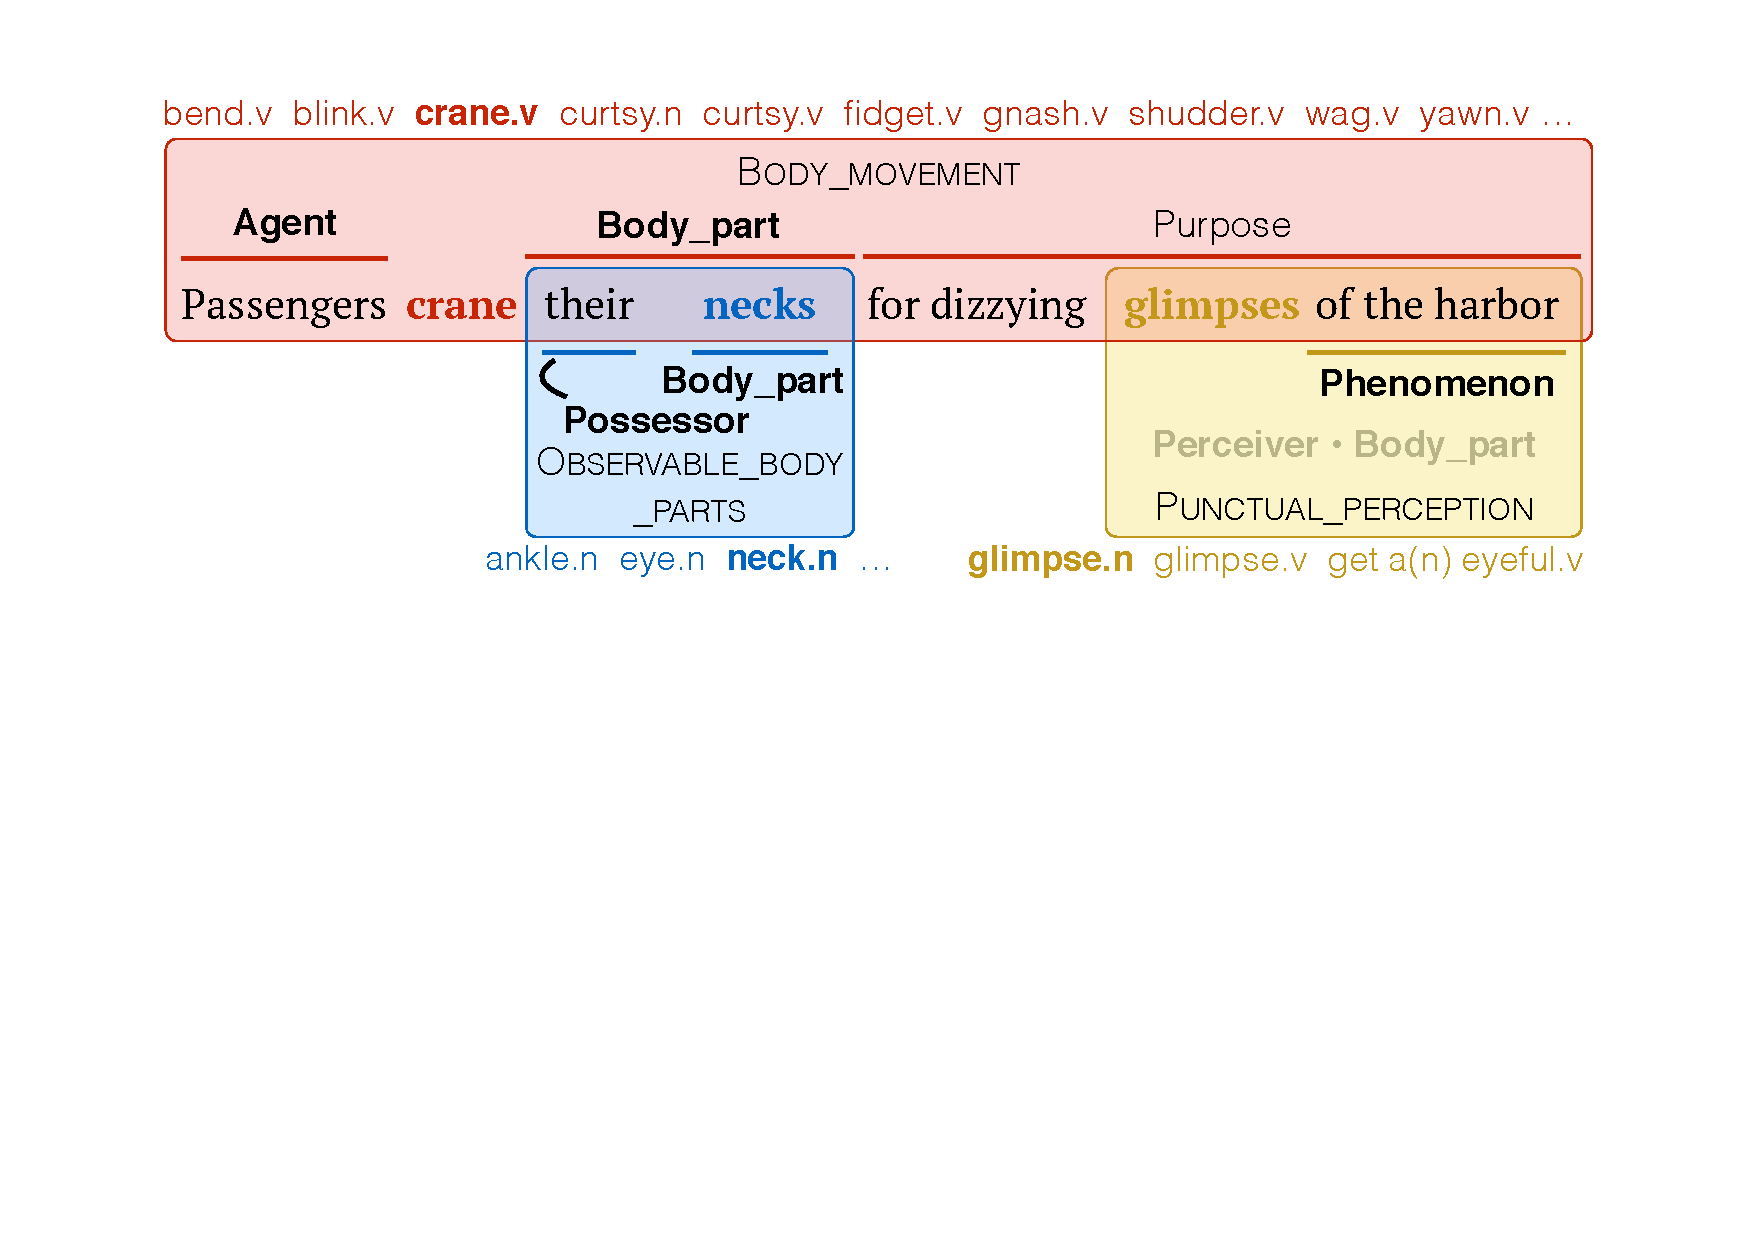
\includegraphics[width=\columnwidth]{fig/harbor-fn.pdf}
\caption{Example sentence from FrameNet full-text annotation. 
3~frames and their arguments are shown: 
\fnf{Body\_movement} is evoked by \textit{crane},
\fnf{Observable\_body\_parts} by \textit{necks}, 
and \fnf{Punctual\_perception} by \textit{glimpse}.
(Further, \textit{harbor} is annotated as evoking the \fnf{Locale\_by\_use} frame 
and doubles as its sole argument.) 
Horizontal lines representing argument spans 
are labeled with role names.}
\label{fig:harbor-fn}
\end{figure}

FrameNet~1.5 defines a structured taxonomy of over 1,000 frames associated with 12,000~English lexical predicates, 
and also provides annotations for over 175,000 attestations 
of these frames/predicates in corpora, annotated in context with their arguments. 
A smaller number of sentences (about 5,000)
are provided with \textbf{full-text} annotations, i.e.~each sentence 
has been analyzed for all available frames. 
But the bulk of sentences in FrameNet---the lexicographic \textbf{exemplars}---are annotated for only one frame per sentence, 
and have thus far not been exploited successfully for the SRL\st{not defined yet} phase of the contemporary frame-semantic parsing task.
Here, we seek to leverage these exemplar sentences 
as well as the (type-level) hierarchical structure of the FrameNet lexicon. 

\begin{figure}
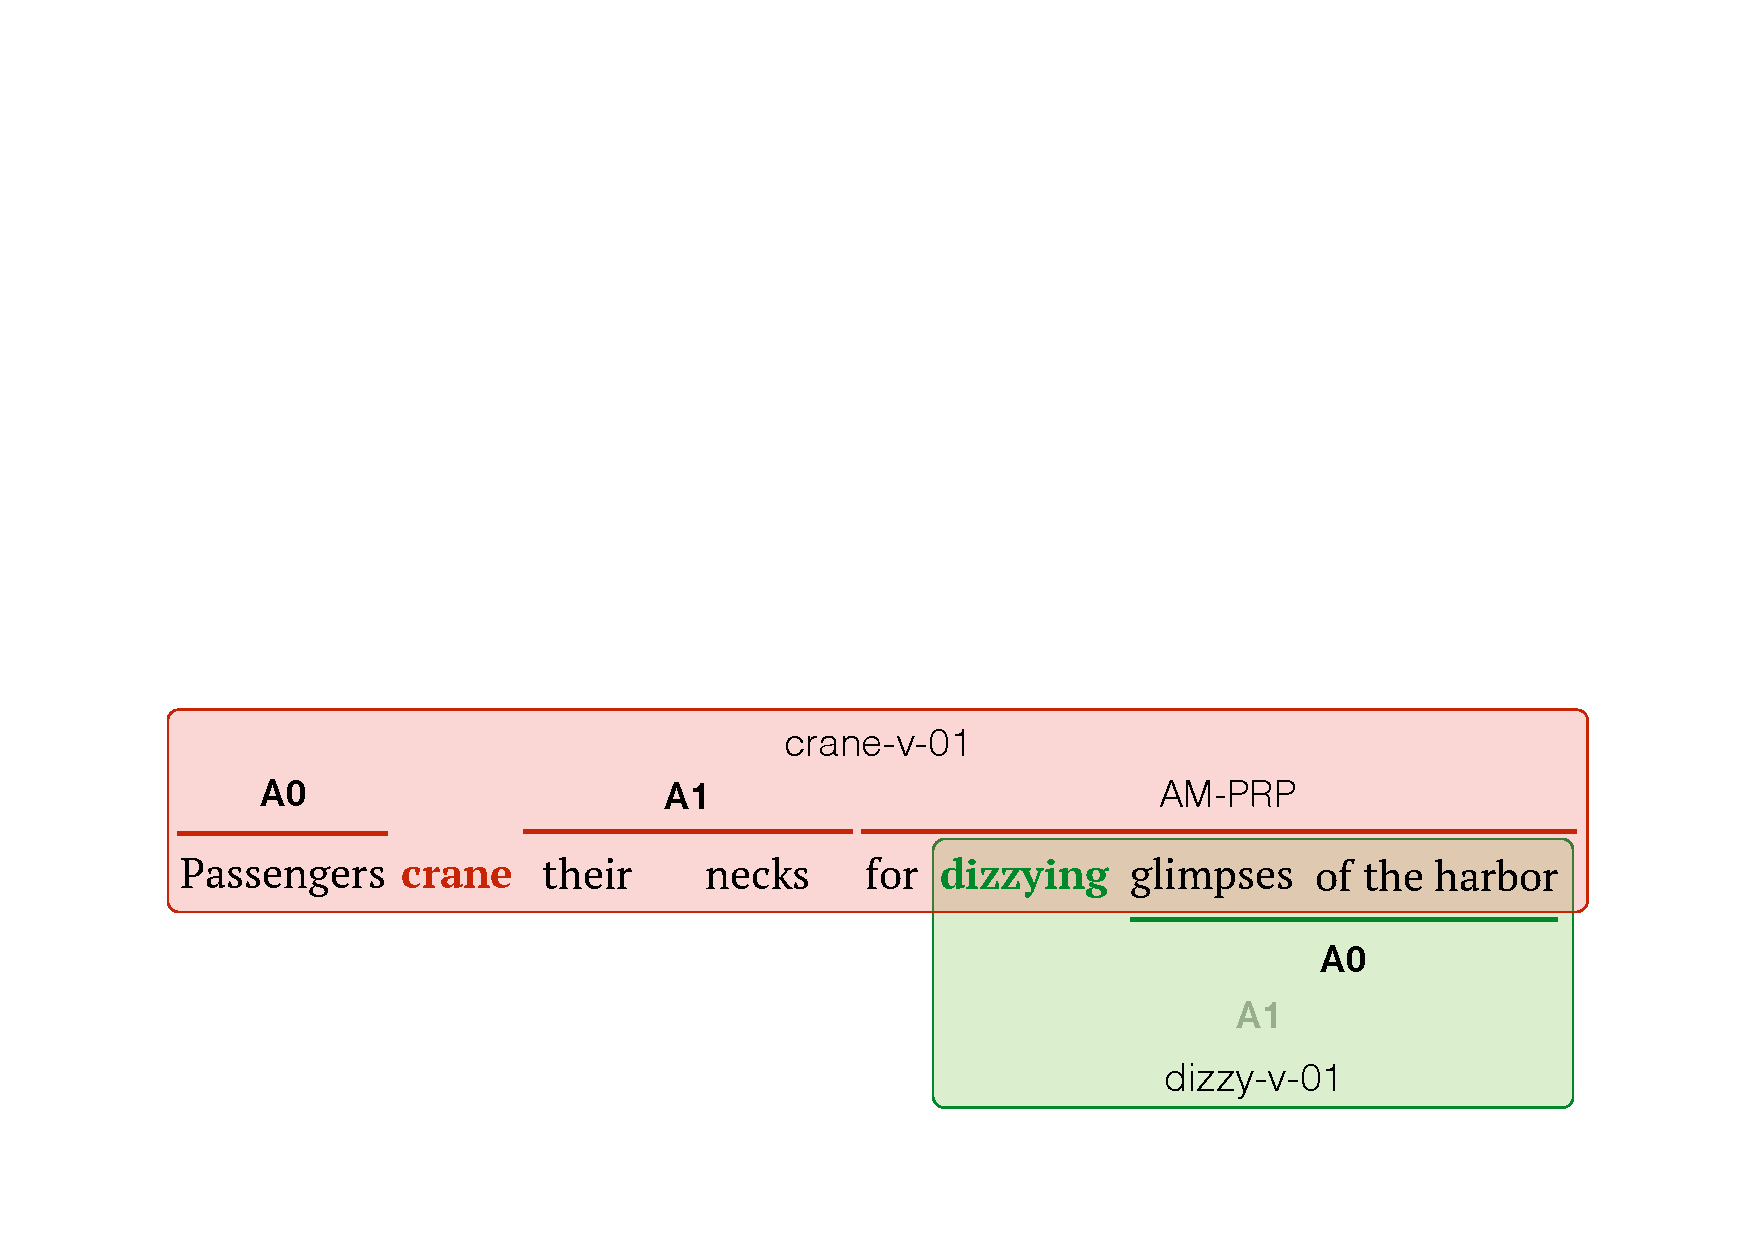
\includegraphics[width=\columnwidth]{fig/harbor-pb.pdf}
\caption{Ideal PropBank annotations for verbs. Though PB uses lexical frames rather than deep frames,
there are clear similarities to the FrameNet annotations in \cref{fig:harbor-fn}.}
\label{fig:harbor-pb}
\end{figure}

In this paper, we address the \textbf{argument identification} 
subtask of finding and labeling arguments 
given a predicate in context and the frame it evokes.
This is a form of semantic role labeling (SRL), 
a task introduced by \citet{gildea-02} using an earlier version of FrameNet.
Another resource, \textbf{PropBank} \citep{propbank}, has been widely used for SRL \citep{palmer-10}. 
PropBank annotations capture shallower lexical frames and arguments; 
additionally, PropBank provides one million words of fully annotated English sentences.
% (annotation is less expensive, but potentially less valuable because of the shallower representation).
Despite a number of differences in the representations and annotation conventions, 
for many predicates FrameNet and PropBank are quite similar: 
\cref{fig:harbor-fn} and \cref{fig:harbor-pb} show this for the verb \textit{crane}.
To get the best of both worlds, we aim to tap into PropBank's vast resources 
as indirect token-level supervision for FrameNet-style analysis. 
We hypothesize that PropBank analyses can serve as a signal for the FrameNet SRL task, either by heuristically transforming PropBank annotations into FrameNet annotations to augment the training data, or by preprocessing sentences with a PropBank SRL system to obtain new features for FrameNet argument identification.

Our experiments expand the \emph{training data} and the \emph{feature space}
of supervised argument identification
in order to integrate evidence from all of these sources 
into SEMAFOR \citep{das-14}, the leading open-source frame-semantic parser for English.\footnote{\url{http://www.ark.cs.cmu.edu/SEMAFOR/}} 
The results show that some of these sources of evidence succeed 
at boosting argument identification performance.\nss{SOTA (without constraints)?}


\section{Resources}

\nss{incl. data analysis of differences from full-text}

\nss{w/in each mention: genre/overall vocabulary; coverage and distributions of predicates, FE labels; oracle coverage of FT test}

\subsection{The FrameNet Lexicon}\label{sec:lex}

Each frame in the Berkeley FrameNet lexicon is intended to represent a gestalt scene. 
The frame definition includes: a descriptive name; 
a set of \textbf{core roles} representing participants and props that are crucial 
to understanding the scene; a set of \textbf{non-core roles} such as circumstantial 
information (time, place, manner, purpose, etc.); 
an English textual description of the scene and how its roles relate to one another;
and a set of English predicates that can evoke the scene.
For example, the \fnf{Body\_movement} frame has \fnr{Agent} and \fnr{Body\_part} as its core roles; 
%the frame description states,
%``This frame contains words for motions or actions an \fnr{Agent} performs using some part of his/her body.''
Lexical entries in this frame include verbs such as \fnlu{bend}, \fnlu{blink}, \fnlu{crane}, and \fnlu{curtsy}, 
plus the noun use of \fnlu{curtsy}.

The frame lexicon is organized as a network, with several kinds of \textbf{frame-to-frame relations} 
linking pairs of frames and (subsets of) their arguments \citep{ruppenhofer-10}. 
Among these kinds of frame-to-frame relations are:\\
\paragraph{Inheritance:} E.g., \fnf{Punctual\_perception} (e.g., \fnlu{glimpse.v}) inherits from 
\fnf{Perception\_experience} (e.g., \fnlu{see.v}), which inherits from \fnf{Perception}. 
%Other frames inheriting from \fnf{Perception} include \fnf{Sensation} (e.g., \fnlu{sight.n}) and 
%\fnf{Becoming\_aware} (e.g., \fnlu{notice.v}). 
Crucially, roles in inheriting (conceptually more specific) frames are mapped 
where they correspond to a role in the inherited frame: so \fnf{Punctual\_perception}.\fnr{Perceiver} links to \fnf{Perception\_experience}.\fnr{Perceiver\_passive}, 
which links to \fnf{Perception}.\fnr{Perceiver}, which links to \fnf{Sensation}.\fnr{Perceiver\_passive} and \fnf{Becoming\_aware}.\fnr{Cognizer}.

\paragraph{Subframe:} This indicates a subevent within a complex event. 
E.g., the \fnf{Criminal\_process} frame groups together subframes 
\fnf{Arrest}, \fnf{Arraignment}, \fnf{Trial}, and \fnf{Sentencing}. 
\fnf{Criminal\_process}.\fnr{Defendant}, for instance, is mapped to 
\fnf{Arrest}.\fnr{Suspect}, %\fnf{Arraignment}.\fnr{Defendant}, 
\fnf{Trial}.\fnr{Defendant}, and \fnf{Sentencing}.\fnr{Convict}. 
Other salient participants in the complex event %(such as the crime for which someone is arrested, tried, etc.)\ 
are similarly mapped via Subframe relations.
This permits an inference that a person tried for a crime likely
has been or will be arrested, arraigned, and sentenced for that crime.

In \cref{sec:hierfeats}, we experiment with features shared between related roles of related frames 
in order to capture statistical generalizations about the kinds of arguments 
seen in those roles and how they relate syntactically to the predicate.

\subsection{Full-text Annotations}\label{sec:ft}

Beginning with the SemEval-2007 shared task on FrameNet analysis \citep{baker-07},
frame-semantic parsers have been trained and evaluated on the \textbf{full-text (FT)}\footnote{Though these 
were \emph{annotated} at the document level, and train/dev/test splits are by document, the frame-semantic parsing 
is currently restricted to the sentence level.} portion 
of the FrameNet corpus. %This consists of documents for which annotators made an effort to assign frames and arguments to as many words as possible. 
\Cref{fig:harbor-fn} gives an example sentence from the FT portion of the corpus. 
It has 4~frame annotations. \fnf{Body\_movement}, as described in the previous section, 
is evoked by \textit{crane}, and 3~of its roles are filled by overt arguments: 
the 2~core roles (\fnr{Agent}, \fnr{Body\_part}) happen to be filled by noun phrases 
(\textit{passengers}, \textit{their necks}), while the non-core role \fnr{Purpose} is filled by a 
prepositional phrase adjunct (\textit{for dizzying glimpses of the harbor}).

\finalversion{The frame defines 19~additional non-core roles, none of which have an argument in the example.
In frame semantics, non-core roles are considered to be \emph{conceptually} optional; 
core roles may or may not be \emph{syntactically} optional, but if not locally specified they are 
expected to be available from context, or else implicit.
For example, \fnf{Punctual\_perception}---evoked in this case by \textit{glimpses}---is annotated 
as missing 2~of its core roles. A human listener would resolve the identity of the \fnr{Perceiver} 
from the wider context and the \fnr{Body\_part} from world knowledge. }

\finalversion{In some cases, FT annotation involved creating a new frame or adding a new lexical unit to an existing frame. 
In other cases, words that in principle should be considered to evoke a frame were left unannotated 
because they did not match any existing lexical units. 
This was the case for \textit{passengers} and \textit{dizzying} in \cref{fig:harbor-fn}.}

The full-text documents represent a mix of genres, prominently including travel guides 
and bureaucratic reports about weapons stockpiles. 
Statistics for the full-text corpus appear in \cref{tbl:datastats}.

\nss{Annotation density: (proportion of tokens evoking a frame. breakdown by POS?)}

\subsection{Exemplars}\label{sec:exemplars}

Conceived primarily as a lexicography project, 
most FrameNet annotations serve to illustrate the argument structure potential 
of particular predicates. When predicates are added to a frame, 
a large set of source corpora (primarily, the British National Corpus) covering a wide range of genres
is searched for various syntactic patterns, 
and a lexicographer identifies a selection, or \textbf{subcorpus}, of sentences 
illustrating the predicate's behavior \citep{boas-05}.
The subcorpus sentences are then annotated, but \emph{only with respect to the predicate in question}.
These singly-annotated sentences are called lexicographic \textbf{exemplars}.

The subset of exemplars containing argument annotations is described in \cref{tbl:datastats}.
Relative to the full-text dataset, the exemplar dataset contains 
an order of magnitude more frame annotations and two orders of magnitude 
more sentences annotated.
Because we are conditioning on the identified frame, 
the fact that the exemplar dataset has just one annotated frame per sentence
is not a concern in argument identification. However, the rate of overt arguments per frame 
is noticeably higher for exemplars, which potentially biases the model's 
tendency to predict certain kinds of arguments in a way that is not statistically representative of a natural corpus.

The exemplar sentences formed the basis of early studies of frame-semantic role labeling \citep[e.g.,][]{gildea-02,thompson-03,fleischman-03,kwon-04}.
We deem it worthwhile to (a)~investigate whether the exemplars 
can be used to improve performance on the full-text evaluation, 
compensating for the scarcity of full-text training data,
and (b)~to evaluate SRL performance on a held-out set of exemplars, 
given that these exemplars represent a much broader range of genres, frames, and predicates 
than the full-text data.
This second evaluation, we believe, will give a useful indication of the robustness of the SRL model.

\subsection{PropBank}\label{sec:pb}

PropBank \citep[PB;][]{palmer-05} is a lexicon and corpus of predicate--argument structures
that takes a shallower approach than FrameNet. Whereas FrameNet frames cluster 
lexical predicates that evoke similar kinds of scenarios (with the same kinds of roles), 
and these frames are organized in a network, 
PropBank frames are purely lexical and there are no formal relations between different predicates 
or their roles. Further, PropBank's sense distinctions are generally coarser-grained than FrameNet's.

\finalversion{PropBank does represent lexical ambiguity---e.g., the verb \textit{order} is ambiguous 
in PropBank between \pbf{order-v-01} ``impelled action'' and \pbf{order-v-02} ``request to be delivered''---but
PropBank's sense distinctions are generally coarser-grained than FrameNet's.}

%Within sense-disambiguated PropBank frames, or \textbf{rolesets}, 
Core roles are defined with textual descriptions and assigned numbers. 
E.g., \pbf{order-v-02} defines: \pbr{A0} ``orderer'', 
\pbr{A1} ``thing ordered'', \pbr{A2} ``benefactive, ordered-for'', 
and \pbr{A3} ``source''.
Following \citeposs{dowty-91} theory of proto-roles, PropBank rolesets use \pbr{A0} for proto-agents 
and \pbr{A1} for proto-patients, but in general, there is much less consistency 
in interpretation of core roles across lexical predicates for PropBank than there is for FrameNet.
Another difference is that PropBank's non-core roles---named \pbr{AM-*}, 
such as \pbr{AM-PRP} for purposes---are not frame-specific.\footnote{\Citet{ellsworth-04} 
has a more extensive discussion of differences between PropBank's and FrameNet's conventions.}

Despite all these differences, there is often a great deal in common between 
FrameNet-style and PropBank-style analyses, as should be apparent from comparing 
\cref{fig:harbor-fn} and \cref{fig:harbor-pb}. 
The major benefit to PropBank is that it includes a large and comprehensively annotated corpus.
We hypothesize that leveraging this large corpus indirectly 
can reap rewards for FrameNet-style SRL. 

Very little data is annotated with both PropBank and FrameNet analyses.
Therefore, to bridge between the PropBank and FrameNet corpora, 
we explore two approaches: (a)~running a PropBank-trained semantic role labeler 
on the FrameNet data as an additional form of preprocessing; and 
(b)~leveraging SemLink \citep{bonial-13}, a partial and semi-automatic augmentation 
of the PropBank corpus's roleset annotations with mappings to FrameNet and VerbNet.

\section{Learning from multiple domains and representations}

We use the model from SEMAFOR \citep{das-14}, described in \S\ref{sec:base_model}, as a starting point.
We experiment with several domain adaptation (DA) techniques, augmenting the model's training data (\S\ref{sec:aug_data}) and feature space %$\mathbf{\phi}$
(\S\ref{sec:frust}--%,\ref{sec:frust},\ref{sec:guide},
\ref{sec:hierfeats}).
% modifying the model-fitting portion of the argument identification model's local learning objective  (training data, features).


\subsection{Base model}
\label{sec:base_model}

The argument identification task is treated as a structured prediction problem.
% We consider the argument identification task as statistical classification 
% for each role of the frame in context.
Let the classification input be a dependency-parsed sentence $\mathbf{x}$, 
the token(s) $p$ constituting the predicate in question, and the frame $f$ evoked by $p$
(as determined by frame identification). 
We use a heuristic procedure \st{cite} for extracting candidate argument spans 
for the predicate; call this $\textit{spans}(\mathbf{x}, p, f)$.
$\textit{spans}$ always includes a special span denoting an empty or non-overt role, denoted $\emptyset$. 
For each candidate span $a \in \textit{spans}(\mathbf{x}, p, f)$, we extract a binary feature vector 
$\mathbf{\phi}(a, \mathbf{x}, p, f)$.
We describe the features in \S\ref{sec:features}.\st{are we going to describe the baseline semafor features?}\nss{i suggest just mention the kinds of things features look at---POS, syntax, etc.---and that many of them are at multiple levels of granularity (role-specific, role name--specific)}
We use a linear model, parametrized by the weight vector $\mathbf{w}$, to score $a$:
\begin{equation}
\textit{score}_\mathbf{w}(a \mid \mathbf{x}, p, f, r) = \mathbf{w}^\top \mathbf{\phi}(a, \mathbf{x}, p, f, r)
\end{equation}
$\textit{score}_\mathbf{w}$ models the compatibility  of a candidate
role--argument pair, and its parameters (feature weights) $\mathbf{w}$ are
learned from data (\S\ref{sec:learning}).

At inference time, we use a \term{global classifier}.
The global classifier chooses a joint assignment of all arguments of a frame, while respecting the following constraints:
\begin{enumerate}
  \item a role may be assigned to at most one span, and
  \item spans of overt arguments must not overlap.
\end{enumerate}
Formally, let a joint assigment be represented as a function $\mathbf{a}: \textit{roles}(f) \rightarrow \textit{spans}(\mathbf{x}, p, f)$, % \cup \{\emptyset\}$, %= \{ (r, a) \mid r \in \textit{roles}(f) \}$
 and let $\mathcal{A}$ be the set of all non-overlapping joint assignments.
We give $\mathbf{a}$ the score:
\begin{equation}
\textit{score}_{\mathbf{w}}(\mathbf{a} \mid \mathbf{x}, p, f) =
    \sum_{r \in \textit{roles}(f)}{\textit{score}_\mathbf{x}(\mathbf{a}(r) \mid \mathbf{x}, p, f, r)}
\end{equation}
and choose the joint assignment:
\begin{equation}
\label{eq:args}
\textit{args}(\mathbf{x}, p, f) =
    \argmax_{\mathbf{a} \in \mathcal{A}} {
        \textit{score}_{\mathbf{w}}(\mathbf{a} \mid \mathbf{x}, p, f, r)
    }.
\end{equation}
Beam search, with a beam size of 100, is used to find this $\argmax$.%
\footnote{Recent work has improved upon global decoding techniques \citep{tackstrom-15}.
We expect such improvements to be complementary to the gains due to the added features and data reported here.}

\mk{introduce this as a supervised domain adaptation problem? What is the source and what's the target?}
\mk{Let $D_{ft}$ represent the FT data and $D_{ex}$ the exemplars?}


\nss{Domain adaptation/multitask learning techniques}

\subsection{Augmenting the Training Data}
\label{sec:aug_data}

This is the simplest possible technique:
we add the exemplars training data, $\mathcal{D}_{ex}$, to the full text training data, $\mathcal{D}_{ft}$, without differentiating between the two, and train on the combined dataset.

\subsection{Frustratingly Easy}
\label{sec:frust}
\Citet{daume-07} proposed a simple feature augmentation approach that was shown to work well in supervised domain adaptation scenarios, 
such as ours.
We %apply their method to incorporate the exemplars data  by introducing
introduce a domain indicator %$I_{\textit{domain}}(\mathbf{x}) =
$\indicator{\mathbf{x} \in \mathcal{D}_{ft}}$,
where $\indicator{P}$ is the indicator function, with value 1 if $P$ is true, 0 otherwise.
% \[
% \indicator{P} = \left\{\begin{array}{lr}
% 1, & \text{ if } P \\
% 0, & \text{ otherwise}. \\
% \end{array}
% \right.
% \]
We expand the feature space by concatenating the original feature vector with a version of the feature vector that has been element-wise conjoined with the domain indicator:
% We apply their method to incorporate the exemplars data  by introducing a feature mapping $\Phi : \mathds{R}^d \rightarrow \mathds{R}^{2d}$ given by
% \begin{equation}
% \Phi(\mathbf{\phi}(a, \mathbf{x}, p, f, r)) = [x; x * ]
% \end{equation}
%  for the
\begin{align*}
\lefteqn{
\phi_{\textit{frust}}(a, \mathbf{x}, p, f, r) =
} \\
&&
\left[\begin{array}{c}
\phi(a, \mathbf{x}, p, f, r) \\
\phi(a, \mathbf{x}, p, f, r) \text{ \& } \indicator{\mathbf{x} \in \mathcal{D}_{ft}}%I_{\textit{domain}}(\mathbf{x})
\end{array}
\right]
% \left[\phi(a, \mathbf{x}, p, f, r) ; \phi(a, \mathbf{x}, p, f, r) \wedge I_{\textit{domain}}(\mathbf{x}) \right]
\end{align*}
\st{this ``vector concatenation'' view is sort of inconsistent with the ``adding features" view in the guide/hierarchy sections}

% FT annotations $x \in \mathcal{D}_{ft}$, and $\Phi^{ex}(x) = (x, 0)$ for the exemplars $x \in D_{ex}$. The resulting transformed data 
% from the two domains is then used to learn a single model.
The intuition is that by replicating the features, we allow for
each feature to contribute both ``general'' and ``domain-specific'' weights to the model depending on whether the feature
behaves similarly in both domains or not.
Since the general feature contributes to both domains, regularization will encourage the model to use the general version over the domain-specific version of a feature whenever possible.

\subsection{Guide Features}
\label{sec:guide}
Another approach to introduce supervision for domain adaptation %, 
% which does not combine the labeled data from the two domains, 
is to train a supervised model on a source domain, make predictions using that model on the training data of the target domain, then use those predictions as additional features while training a new model on the target domain.
% is to use a supervised model built on the source domain to augment features in the target domain.
% When training and testing in the target domain, 
The source domain model is effectively a form of preprocessing, and the features from its output are known as \textbf{guide features} \citep{johansson-13,kong-14}.\footnote{This is related to the technique
of model stacking, where successively richer models are trained by cross-validation on the same dataset 
\citet[e.g.,][]{cohen-05,nivre-08,martins-08}.}

In our case, we treat the full text annotations as our target domain, and experiment with using PropBank, SemLink, and the exemplars data as source domains.
Each of the three source models produces SRL-style output, where predicates are assigned frames or rolesets, and for each predicate, spans are assigned role labels.
But they differ in the labels used for roles.
\st{talk about Illinois SRL \citep{punyakanok-08}\footnote{\url{http://cogcomp.cs.illinois.edu/page/software_view/SRL}}, whatever-we-did-with-SemLink here?}

Formally, let $M_{s}$ be the model built on
the source domain (for instance, the PropBank data). 
For every target domain sentence $\x$, we introduce ``guide'' features which use the output $M_s(\x)$
obtained by applying $M_s$ on $\x$, which consists of the role labels assigned to various text spans in $\x$.
Two types of guide features were used:
one indicates that a span $a$ was assigned \emph{any} role, and the other encodes the role label $r_g$ itself.
In the case where $M_s$ produces labels
that belong to the same schema as the target domain 
(for instance, the exemplars use the same schema as the FT annotations \st{our set of source domains is small enough that we can enumerate which ones this applies to. Is it exemplars + SemLink?}), 
we use an additional feature $\phi_{match}(r_t,r_g)$ to indicate that 
the `guide' role label $r_g$ of the span $a$ is the same as it's true\st{you mean ``target''?} label $r_t$.


\subsection{Type-level hierarchy features}\label{sec:hierfeats}
\mk{NSS: notation for the frame/role/features etc?}
\mk{How many total types of relations? Cleanup writeup based on NSS's notation.}

Frames in FrameNet are connected to each other by relations such as inheritance, temporal ordering, causality. 
For instance, the frame \fnf{Robbery} inherits from the more abstract frame \fnf{Committing\_crime}, and the
frame \fnf{Fall\_asleep} is preceeded by the frame \fnf{Being\_awake}. The roles of related frames have 
also been mapped to indicate the correspondence between them: \fnf{Robbery}.\fnr{Perpetrator} is mapped to 
\fnf{Committing\_crime}.\fnr{Perpetrator}, which in turn maps to \fnf{Misdeed}.\fnr{Wrongdoer}. Frames and roles that are far
apart in this hierarchy are less related than say neighbours.
This hierarchy can be exploited to share information across related roles, thereby benefiting the roles 
that have few annotations \mk{say something about a greater variety of contexts is available for each role}. 
We say that the $\textit{parent}$ of a role is one that has either the \textbf{Inheritance} or \textbf{Subframe} relation to it (\cref{sec:lex}).
There are 4138 \textbf{Inheritance} and 589 \textbf{Subframe} links between role types in FrameNet 1.5.

A simple mechanism to share information is via shared model parameters between related roles. Towards this, we experiment with two variations of
hierarchical feature types:

\begin{itemize}
  \item 
\noindent\textbf{siblings}: Roles that have a common parent share features.
For every feature $\phi_i(a, \mathbf{x}, p, f, r)$, we add a new feature which is the conjunction: 
$\text{"sib"} \wedge \phi_i(a, \mathbf{x}, p, f, r) \wedge \textit{parent}(r)$. 
% $I_{hier}$ is an indicator to distinguish this feature from the regular conjunction features in Semafor that use frame names and roles.

  \item\noindent\textbf{parent+siblings}: Roles share features with their parent and siblings. 
For every feature $\phi_i(a, \mathbf{x}, p, f, r)$, we add a two new features:

\noindent$\text{"par+sib"} \wedge \phi_i(a, \mathbf{x}, p, f, r) \wedge \textit{parent}(r)$, and

\noindent$\text{"par+sib"} \wedge \phi_i(a, \mathbf{x}, p, f, r) \wedge r$.
\end{itemize}

We experimented with using more than one level of the hierarchy (grandparents, e.g.), but found that it does not produce any improvements in the performance, yet increased computation cost due to the greater number of features.



\section{Experiments}

All of our experiments use the same form of regularization, 
condition on the same oracle frame predictions, 
and syntactic preprocessing\nss{does this match Dipanjan's latest experiments?}, 
and use beam search with a beam size of 100 for joint decoding of the test data.
Automatic syntactic dependency parses from MSTParserStacked \citep{martins-08} are used, as in \citet{das-14}. % to narrow the set of candidate spans considered, and as input to feature extraction.


\subsection{Learning}
\label{sec:learning}

Following SEMAFOR, we train using a \term{local} objective instead of using a global classifier.
In other words, we treat each role and span pair as an independent training instance.
% SEMAFOR treats the argument identification task as a structured prediction problem.
% It uses a linearly parametrized model that scores each candidate span given a frame element\st{this should probably be talked about earlier?}:
% \begin{equation}
% \textit{score}_\mathbf{w}(y \mid x) = \mathbf{w}^\top \mathbf{f}(x, y)
% \end{equation}
%
% During training, each frame element is treated as an independent log-linear classification instance, with the set of candidate spans (including the \textsc{NULL} span) as its output space.
% \st{something about L2 regularization}
% But at test time, it chooses a joint assignment of all arguments that maximizes probability under the model, while satisfying the following constraints:
% \begin{enumerate}
%   \item an argument may be assigned to at most one span \st{theta criterion, Chomsky}, and
%   \item spans of realized arguments must not overlap.
% \end{enumerate}
% Beam search, with a beam size of 100, is used to choose the maximum joint assignment with no overlapping arguments.
% \nss{does beam search require normalizing to probabilities?}\st{no. maybe it should, but SEMAFOR didn't, and we don't.}
But we have made several modifications to SEMAFOR's training in order to speed up experiments:

\begin{itemize}
  \item We minimize squared structured hinge loss (defined below) instead of a log-linear loss.
  Using hinge loss, there is no longer a need to calculate a partition function.
  Gradients, and hence parameters, are sparser than in a log-linear model, as they only depend on the correct span and the predicted span.
  \item We use the online optimization method AdaDelta \citep{zeiler-12} with minibatches, instead of the batch method L-BFGS \citep{liu-89}.
  We use minibatches of size 4,000  on the full text data, and 40,000 on the exemplar data.
%   \item We use elastic net ($\ell_1 + \ell_2$) regularization. Adding $\ell_1$ also has the effect of keeping the parameter vector sparse.\nss{what hyperparameter(s)? are $\ell_1$ and $\ell_2$ tuned separately?}
\end{itemize}
We use these changes for all systems, including the baseline.
While the impact on full-text performance is negligible, 
these changes enabled us to run more experiments with the larger exemplar dataset and expanded feature space.\footnote{With SEMAFOR's original features and training data, 
the result of the above changes is that full-text $F_1$ decreases from 59.3\% to 59.1\%, 
while training time (running optimization to convergence) 
decreases from 729 minutes to 82 minutes\nss{say something about hardware this was tested on?}.%
%\mk{P/R/F numbers are in the table (see rows 1 and 2). Times: 12 hrs 9 mins for the earlier algorithm to converge. That took 290 iterations. An equivalent number of iterations took 45 minutes for the new system. Running till convergence (about 700 iterations) took 82 minutes, thus giving a speed-up of $\approx$ 9X. The P/R/F on exemplars improves (row 2); I believe it is due to the regularization in Sam's objective.}
} 

% \st{TODO: local classifier is only used in my SVM version, not in Das's log-linear version.}
% We define the \textbf{local classifier} as:
% \begin{equation}
% \textit{arg}(\mathbf{x}, p, f, r) = \argmax_{a \in \textit{spans}(\mathbf{x}, p, f)
% } \textit{score}_{\mathbf{w}}(a \mid \mathbf{x}, p, f, r)
% \end{equation}
% 
% \st{something about L2 regularization}

The details of squared hinge loss are as follows.

Let $((\mathbf{x}, p, f, r), a)$ %$(r^{(i)}, a^{(i)})$
be the $i^{\text{th}}$ training example.
Then the structured hinge loss on the $i^{\text{th}}$ example is given by:
\begin{align*}
\lefteqn{\textit{Hinge}_\mathbf{w}(i) =} \\
&&\max_{a^\prime}{\{\mathbf{w}^\top \mathbf{\phi}(a^\prime, \mathbf{x}, p, f, r) + \text{cost}(a^\prime, a)\}} - \\
&&\mathbf{w}^\top \mathbf{\phi}(a, \mathbf{x}, p, f, r)
\end{align*}
and squared hinge loss is:
\begin{equation}
\textit{SqHinge}_\mathbf{w}(i) =
\textit{Hinge}_\mathbf{w}(i)^2.
\end{equation}
We use $\text{cost}(a^\prime, a) = \indicator{a^\prime \ne a}$.%
\footnote{We experimented with recall-oriented training, where errors of omission are assigned a higher cost, but found that while recall increased, overall $F_1$ went down\nss{or: failed to improve?}.}

We learn $\mathbf{w}$ by minimizing the $\ell_2$-regularized average loss on the dataset:
\begin{equation}
\mathbf{w^*} = \argmin_\mathbf{w}{
    \frac{1}{N}\sum_{i = 1}^N\{
        \textit{SqHinge}_\mathbf{w}(i)
    \} + \frac{1}{2} \lambda \| \mathbf{w} \|_2^2
}
\end{equation}





\subsection{Preprocessing the Data}
\ref{sec:preproc}

\paragraph{Full-Text.}
For the FT annotations, we use the same FrameNet 1.5 data and train/test splits as \citet{das-14}, without any of our own processing.

\paragraph{Exemplars.} 
We processed the exemplars data (\cref{sec:exemplars}) to remove sentences which had no role annotations (under the assumption that these are likely to be
incomplete annotations). Out of a total of 145838 sentences, $\approx$4000 had only frame annotations. 
We further removed duplicate sentences that already appear in the FT data. 
In the argument annotations, we merged spans which were adjacent and had the same argument label.

\paragraph{SemLink.} 
SemLink (see \cref{sec:pb}) contains two types of mappings. The \emph{sense-level mappings} give correspondences between the concepts
from each resource---i.e., between `frames' from FN, `rolesets' from PB, and `roles' from VN. 
Since they map different interpretations and granularities 
of concepts, the sense-level mappings may be one-to-one, one-to-many, or many-to-many.
PropBank and FrameNet are mapped indirectly via VerbNet. %, introducing additional coverage gaps and ambiguities.
Second, SemLink provides some \emph{token-level parallel annotations} 
for the 3~representations in a subset of the PB-WSJ text: hereafter SL-WSJ.

We focus on using token-level SemLink version~1.2.2c annotations as a (disambiguated) mapping from PB to FN tokens.
Of the available 74,977 SL-WSJ verbs, a majority cannot be mapped to FN frames for various reasons.
Around 31\% of the predicates have the frame label \texttt{IN} (``indefinite'') where the mapping from VerbNet to FrameNet is ambiguous.
About 20\% of the instances are labeled \texttt{NF} (``no frame''), indicating a coverage gap in FrameNet. 
21\% of verbs have frame labels but no frame element annotations. Most of these are predicates with modifier arguments.
Other arguments pointed to null anaphora that could not be resolved to overt arguments.
This leaves 15,323 mappable instances with at least one overt argument, or 20\% of SL-WSJ verbs. This is a very small
subset of the entire PB annotated data.

Some of the FN information in SemLink is out of date due to subsequent changes in FrameNet.
There are some erroneous FN annotations as well: e.g., all 14~instances of \vpred{liquidate} are
labeled \fnf{Killing}, despite being used in the financial sense; and in 17~cases \vpred{direct}
is erroneously marked as \fnf{Behind\_the\_scenes} (i.e., film direction).
These kind of errors are hard to detect and remove.


\nss{OntoNotes PropBank preprocessing (NLTK)?}

\subsection{Hyperparameter Tuning}

We tune the $\ell_2$ regularization parameter $\lambda$ on the FT dev set, searching over the following
values: 10$^{-5}$, 10$^{-7}$, 10$^{-9}$, 10$^{-12}$ (note that our loss is normalized).
We also use the performance on the FT dev set to determine the stopping criterion for the stochastic optimization. The FT dev set was used 
only to tune parameters and not as part of the model construction. 
%Also note that we do not tune any parameters w.r.t the exemplars data.
%\mk{Do I need to mention this -- The model with the best performance on the FT dev set is used for all evaluation}



\subsection{Evaluation}
A complete frame-semantic parsing system involves two main steps: frame identification and argument identification. Since the focus of this work is only 
argument identification, we assume that the gold-standard frames are given and evaluate the models on their role labeling performance.
The baseline model from \citet{das-14} that we compare against, is the current state-of-the-art for argument identification (i.e frame SRL).

The performance of the various methods is compared on two different test sets.
(1) Full-text: the FrameNet 1.5 FT test split that was used in the evaluation in \citet{das-14}. This data consists of sentences from 23 documents. 
(2) Exemplars: a randomly sampled set of sentences from the exemplars data, with approximately the same number of targets as the FT test set.
Statistics of both the test sets are given in the lower half of Table \ref{tbl:datastats}. 
The FT test set has 289 unseen role types, which is much higher than
the 38 in the exemplars test set. There are no unseen frame types in the exemplars test data, whereas the FT test has 46 of them. 
These differences are due to the manner in which the train and test splits were created, with document-level splits being used
for FT and sentence-level splits for the exemplars.
The last row of Table \ref{tbl:datastats} shows the unseen role types faced by a model that was built on both the FT and exemplars training data.
In the FT test set it is 103, lower by $\approx$190 than what a FT-only model will see, thus leading us to expect that a model that combines
both sets of data will certainly benefit in performance.


\begin{table}\centering\small
\begin{tabular}{@{}p{2cm}r@{~~}r@{~~}r@{~~}r@{}}
%\toprule
\normalfont & \multicolumn{2}{c}{\textbf{\hspace{40pt}Full-Text}} & \multicolumn{2}{c}{\textbf{Exemplars}} \\
& \multicolumn{1}{c}{\hspace{40pt}\textit{train}} & \multicolumn{1}{c}{\textit{test}} & \multicolumn{1}{c}{\textit{train}} & \multicolumn{1}{c}{\textit{test}} \\
\midrule
Sentences  & 2,780 & 2,420 & 137,515 & 4,132 \\
Frames & 15,019 & 4,458 & 137,515 & 4,132 \\
Overt args & 25,918 & 7,210 & 278,985 & 8,417 \\
\midrule
\multicolumn{5}{c}{\textsc{types}} \\
Roles & 2,644 & 1,420 & 4,821 & 1,224 \\
\multicolumn{2}{@{}l}{Unseen frames  \quad \textit{vs.~train:}} & 46 & & 0 \\
\multicolumn{2}{@{}l}{Roles in unseen frames \quad \textit{vs.~train:}} & 178 & & 0 \\
\multicolumn{2}{@{}l}{Unseen roles \quad \textit{vs.~train:}} & 289 & & 38 \\
\multicolumn{2}{@{}l}{Unseen roles \quad \textit{vs.~combined train:}} & 103 & & 32 \\
\end{tabular}
\caption{Characteristics of the training and test data. (These statistics exclude the development set, which contains 4,463 frames over 746 sentences.)}
\label{tbl:datastats}
\end{table}

While the FT test set represents the benchmark set for evaluating the 
performance of a frame semantic role labeling system, the exemplars test set being from a different distribution of text, gives us
an indication of how well a model generalizes.

\subsection{Results}

\nss{comparison to prior work (baseline, best result). args+frames score vs. args only}
\nss{be sure to mention: gold frames}
We present precision, recall, and $F_1$-measure microaveraged across the test instances in Table \ref{tbl:results}, for all the approaches that we tried.
The first column classifies the approaches based on what resource we use and the second column indicates what training data was used. 
For each resource (one multi-row in the table) we show results obtained by various methods of combining it with the FT data.
The marker `$\xrightarrow{\text{guide}}$' on some of the methods refers to the feature augmentation discussed in \cref{sec:guide},
`Hier' represents the hierarchical features from \cref{sec:hierfeats} and `EasyAdapt' refers to the frustratingly easy DA model
described in \cref{sec:frust}.%\nss{if using the term EasyAdapt, define it above}

\begin{table*}\centering\small
\begin{tabular}{>{\itshape}clr<{\hspace*{15pt}}rrr@{~~}r@{~~}rrr}
\toprule
\normalfont\textbf{Additional} & \multicolumn{1}{c}{\textbf{Training Configuration}} & \multicolumn{1}{c}{\textbf{Millions of}} & \multicolumn{3}{c}{\textbf{Full-Text}} && \multicolumn{3}{c}{\textbf{Exemplars}} \\
\cline{4-6}\cline{8-10}
\normalfont\textbf{Resource} &  \multicolumn{1}{c}{\textbf{(Features)}} & \multicolumn{1}{c}{\textbf{Features}} & P\hphantom{11} & R\hphantom{11} & $F_1$\hphantom{0} && P\hphantom{11} & R\hphantom{11} & $F_1$\hphantom{0} \\
\midrule
%(Baseline) & FT (Basic) & 66.03 & 53.79 & 59.29 && 64.90 & 33.60 & 44.27 \\
(Baseline) & FT (Basic) & 2.7 & 65.57 & 53.82 & 59.12 && 62.63 & 37.65 & 47.03 \\
\midrule
\multirow{2}{*}{FN Hierarchy} & FT (siblings) & 5.4 & 67.24 & 54.76 & 60.36 && 64.81 & 39.09 & 48.77 \\
          & FT (siblings+parents) & 8.5 & 67.67 & 52.79 & 59.31 && 65.25 & 38.18 & 48.18 \\
\midrule
\multirow{2}{*}{SemLink} & SemLink $\xrightarrow{\text{guide}}$ FT & 3.0 & 64.67 & 54.53 & 59.17 && 60.95 & 38.92 & 47.50 \\
& FT+SemLink & 5.0 & 65.50 & 37.80 & 47.90 && 57.15 & 20.80 & 30.50 \\
\midrule
& Exemplars $\xrightarrow{\text{guide}}$ FT & 3.5 & 65.24 & 55.96 & 60.24 && 67.71 & 48.08 & 56.23\\
Exemplars & FT+Exemplars (Basic) & 13\nss{.?} & 66.06 & 58.23 & 61.90 && 75.44 & 65.11 & \bf{69.89} \\
& FT+Exemplars (EasyAdapt) & 16\nss{.?} & 65.70 & 59.04 & \bf{62.19} && 73.88 & 61.40 & 67.06 \\
\midrule
PB-SRL & PB-SRL $\xrightarrow{\text{guide}}$ FT & 3.6 & 64.96 & 54.83 & 59.47 && 61.38 & 39.14 & 47.80 \\
\bottomrule
\end{tabular}
\caption{Results on two test sets: Baseline vs.~individual other resources. 
Precision, recall, and $F_1$ are given as percentages.}
\label{tbl:results}
\end{table*}

\begin{table*}\centering\small
\begin{tabular}{lr<{\hspace*{15pt}}rrr@{~~}r@{~~}rrr}
\toprule
\multicolumn{1}{c}{\textbf{Training Configuration}} & \multicolumn{1}{c}{\textbf{Millions of}} & \multicolumn{3}{c}{\textbf{Full-Text}} && \multicolumn{3}{c}{\textbf{Exemplars}} \\
\cline{3-5}\cline{7-9}
\multicolumn{1}{c}{\textbf{(Features)}} & \multicolumn{1}{c}{\textbf{Features}} & P\hphantom{11} & R\hphantom{11} & $F_1$\hphantom{0} && P\hphantom{11} & R\hphantom{11} & $F_1$\hphantom{0} \\
\midrule
FT+Exemplars (Hier: siblings) & 34 & 66.00 & 60.40 & \bf{63.07} && 76.14 & 67.71 & \bf{71.70} \\
PB-SRL $\xrightarrow{\text{guide}}$ FT+Exemplars & 17 & 67.36 & 58.79 & 62.80 && 77.15 & 65.47 & 70.83 \\
%FT+Exemplars (PB-SRL, Hier: siblings) \\
\bottomrule
\end{tabular}
\caption{Combining best techniques across resources \nss{TODO}}
\label{tbl:bestTech}
\end{table*}


The baseline $F_1$ on argument identification published in \citet{das-14} on the FT test set includes adding `pseudo' scores for getting gold frames right. 
However, this does not give us a true picture of the performance, hence we choose not to add frame-level scores while computing $F_1$. 
In Table \ref{tbl:results}, the first row corresponds to the state-of-art $F_1$ from \citet{das-14}.

The first resource that we consider is `FN Hierarchy'. We find that adding the sibling-level hierarchical features to the baseline improves 
$F_1$ by 1.2 and 1.7 points on FT-test and exemplars-test respectively,
with benefits to both precision and recall. The `siblings+parents' features which consider two levels of the hierarchy produce unnoticeable benefits,
suggesting that higher levels in the hierarchy can be too general \mk{give example?} and cause very dissimilar roles firing the same hierarchy features.%
\footnote{We also tried adding grandparents and found only minor improvements. Using an expert-pruned hierarchy with relations that are
most likely to help can give greater benefits, and is beyond the focus of this work.}

SemLink, as we remarked in \cref{sec:preproc} is a noisy resource; we see a confirmation for this observation in the performance of the (FT+SemLink) model,
which drops the $F_1$ by a whopping 11.2 and 16.5 points below baseline on FT-test and exemplars, respectively. 
The guide features however modulate the influence
of the SemLink annotations, giving a minor increase over the baseline. 
%\mk{resulting in a graceful but prompt exit for this resource from further consideration.}

With the exemplars resource, we find that the guide features give us a modest improvement of 1.12 in $F_1$ on FT-test, 
while using it as gold-standard training data results in a bigger increase of 2.8 points. 
On the exemplars-test we observe a similar trend, where the (FT+Exemplars) model delivers a massive increase of $\approx$23 $F_1$-points and a 
much smaller increase is seen with the guide features. This contrasts with what we observed for SemLink.
`EasyAdapt', the frustratingly easy DA approach to incorporate the Exemplars
gives a minor increase of 0.3 points on the FT-test but a reduction of 2.8 points on the exemplars-test.

Finally, using the PB-SRL data in the form of guide features also results in small improvements over the baseline. 
Overall we observe that an additional resource that is very similar to the original resource helps more as training data than as a `guide model'.
Whereas the guide features help more when the additional resource is either unreliable (like SemLink) or too distinct (like PB). 
To summarize the results, we find that adding the sibling-level hierarchical features, using Exemplars as gold-standard training data and 
incorporating PB-SRL data in the form of guide features all help in improving the performance over the baseline on both FT-test and exemplars-test.
 
\subsection{Combining all resources}

We pick the techniques that performed best across the resources and combine them in two models. Table \ref{tbl:bestTech} shows the results on these.
Both models use the optimal training data configuration: (FT+Exemplars). The first one integrates the FN Hierarchy using the `siblings' features
and the second integrates PB-SRL data in the form of guide features. These two models outperform the models discussed in Table \ref{tbl:results}.
On both test sets, we find that the model using the hierarchy achieves the best recall, and the PB-SRL guide features result in the 
best precision. %This result is intuitive because we expect the hierarchy to help \mk{insert good explanation here}.
Our best result of 63.07 on the FT test set beats the baseline (59.12) by 3.95 F points.


\begin{figure}[t]
	\begin{subfigure}[b]{0.5\textwidth}
		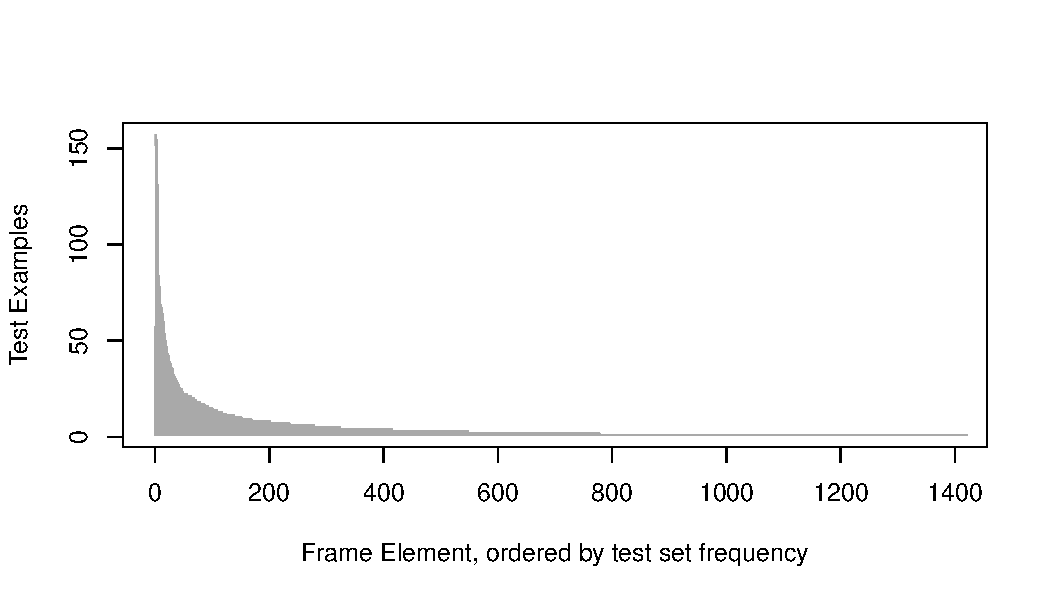
\includegraphics[width=\textwidth]{fig/num_instances}
		\caption{Frequency of each role appearing in the test set.}\label{fig:num_inst}
	\end{subfigure}
	\begin{subfigure}[b]{0.5\textwidth}
		\vspace{-1cm}
		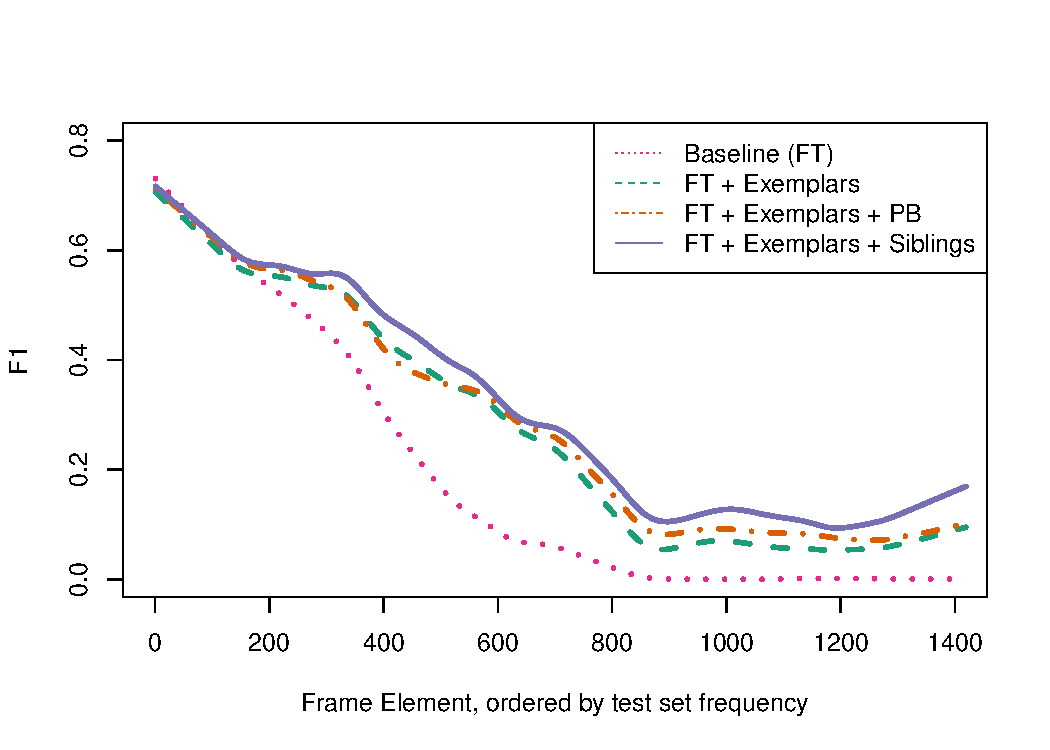
\includegraphics[width=\textwidth]{fig/f1_sorted_by_num_instances}
		\caption{$F_1$ of the best methods compared with the baseline.}\label{fig:coolplot}
	\end{subfigure}
	\caption{Count and $F_1$ for each role appearing in the test set. $F_1$ values have been smoothed with \texttt{loess}, with a smoothing parameter of 0.2.}
\end{figure}

\finalversion{\nss{impact of automatic frames?}}

\subsection{FE-level evaluation}
The results so far have discussed the overall improvement in $F_1$, but do not present a detailed picture of how we gain from the additional
coverage. Towards this, we present a frame-element i.e role type level analysis comparing the best results with the baseline.
The first plot in Figure \ref{fig:num_inst} shows the frequency of all roles that appear in the FT-test set.
Figure \ref{fig:coolplot} shows the $F_1$ per role-type, for the baseline and the two models from Table \ref{tbl:bestTech}.
In both plots, each point on the x-axis represents one role, with the roles sorted in the decreasing order of their frequency.
The $F_1$ curves clearly show that our models achieve the best improvements for the rarer roles and are at par with the baseline on the frequent roles.

\mk{Analyze the sparsity of the models? Which features have highest importance?}
In addition to the performance, we also show the sizes of the various models in the column `Millions of features'.
All the models are quite sparse however,
with $\approx$60-70\% of the features assigned a weight of zero.
The larger models take roughly 6 times as long as the baseline to train. 


\section{Related Work}

Prior work has noted that the preponderance of role labels in FrameNet poses a challenge, and have considered various ways of grouping role labels together in order to share statistical strength. 
\citet{matsubayashi-09} investigated using the \textbf{Inheritance} relationships, and also grouping by the human-readable name of the role, and found small gains from both. Their evaluation was on a simpler subtask of argument classification, and our experiments confirm that their results hold for argument identification as well as classification.
\citet{baldewein-04} use an EM-based clustering method to learn latent groupings of roles and role-fillers, reporting mixed results.
\citet{shi-05} used a rule-based mapping between FrameNet and VerbNet, and between VerbNet and WordNet, and used these mappings to build a semantic parser.

\citet{tackstrom-15} is the most recent work on frame-semantic argument identification.
They present an efficient dynamic program for solving the joint role assignment problem (equation~\ref{eq:args}), and show that using it at training time is helpful.
Their work is complementary to our own.
\citet{das-11,das-12} investigated semi-supervised techniques using the exemplars and WordNet for frame identification.
\citet{hermann-14} also improve frame identification in a way that allows sharing of statistical strength among related frames, by mapping frames and predicates into the same continous vector space.

% \nss{Dipanjan's other papers (focusing on different parts of the task)}
\nss{be sure to cite: \citep{merlo-09} (multiple resources + levels of generalization), \citep{furstenau-09} (semi-supervised)}


\nss{multitask learning?}
\mk{there's no room for citing MTL.. we can do that later}

\section{Conclusion}

We have empirically shown that auxiliary semantic resources
can benefit the challenging task of frame-semantic role labeling.
Complementary gains on the standard full-text evaluation are achieved
by including the FrameNet exemplars in the training data 
and by grouping features according to the FrameNet hierarchy. 
There are smaller, but nevertheless promising, signs that data annotated 
with the PropBank scheme can be leveraged as well.
In addition to making SRL more \emph{accurate}, 
a parallel evaluation on a sample of exemplars suggests the 
improved models are also more \emph{robust}, 
capturing a broader swath of the English language.

We are optimistic that future improvements to lexical semantic resources, 
including planned changes for PropBank \citep{bonial-14} and SemLink \citep{bonial-13}, 
will lead to further gains in this task. 
Moreover, the techniques discussed here could be further explored 
using semi-automatic mappings between lexical resources \citep[such as UBY;][]{gurevych-12}, 
and correspondingly, this task could be used to extrinsically validate those mappings.

\finalversion{\section*{Acknowledgments}

FUNDING}

\smaller

\bibliographystyle{style/aclnat}
% you bib file should really go here
\setlength{\bibsep}{1pt}
{\fontsize{10}{12.25}\selectfont
\bibliography{argid}}

\end{document}
